\problem{Mass-Spring System}

This homework investigates spring equations using the following code:
\begin{verbatim}
function LAB05ex1
m = 1;
% mass [kg]
k = 4;
% spring constant [N/m]
omega0 = sqrt(k/m);
y0 = 0.1; v0 = 0;
% initial conditions
[t,Y] = ode45(@f,[0,10],[y0,v0],[],omega0); % solve for 0<t<10
y = Y(:,1); v = Y(:,2);
% retrieve y, v from Y
figure(1); plot(t,y,'b+-',t,v,'ro-');
% time series for y and v
grid on;
% Legend!
legend('y(t)', 'v(t)');
%-----------------------------------------
function dYdt = f(t,Y,omega0)
y = Y(1); v = Y(2);
dYdt = [ v ; -omega0^2*y ];
\end{verbatim}

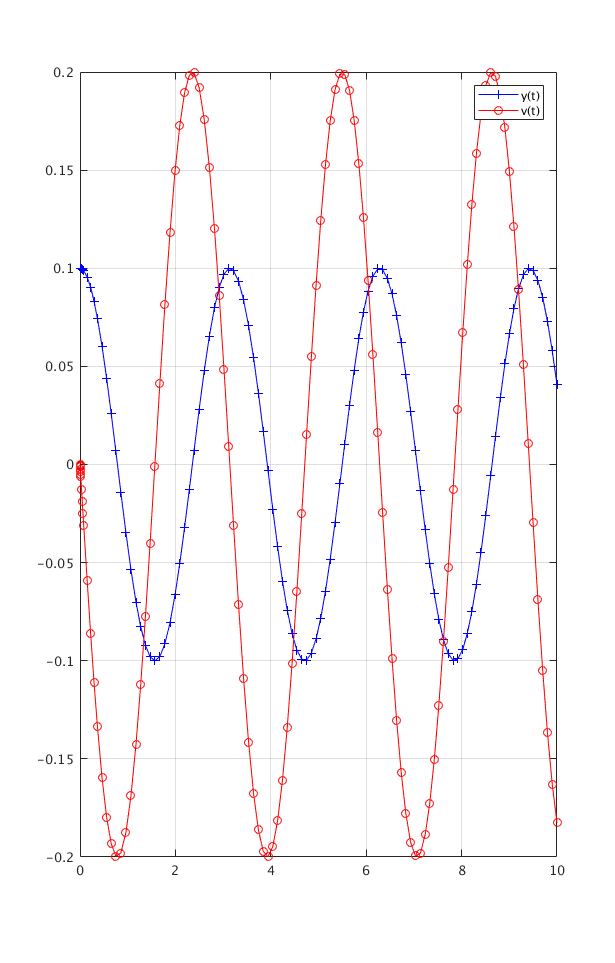
\includegraphics[width=4in, scale=0.4]{0.png}

\solution
\begin{itemize}

\item (a) Which curve represents $y = y(t)$? How do you know? \\ 
    The blue curve represents $y = y(t)$. This is because it starts at $y0 = 0.1$, while $v$ (the red curve) starts at $0$, and represents the derivative of $y$ with respect to $t$.
\item (b) What is the period of the motion? Answer this question first graphically (by reading the period from the graph) and then analytically (by finding the period using $\omega_0$). \\
    Visually, the period appears to be roughly $\pi$, starting from $2.39$ in the matlab graph. This can be verified by using the equation for the period of the spring, $T=2\pi \sqrt{\frac{m}{k}}$, i.e. $\frac{2\pi}{\omega_0}$. Since $\omega_0$ is $2$, $T$ is $\pi$.
\item (c) We say that the mass comes to rest if, after a certain time, the position of the mass remains within an arbitrary small distance from the equilibrium position. Will the mass ever come to
rest? Why? \\
The mass will never come to rest, because there is no dampening. Essentially, this comes down to being unable to take the limit of $y$, since, for any arbitrary end value, increasing the value can yield a different value of $y$. We know there is no dampening because the amplitude appears to be constant. Later in the homework (in an unrequired question), a different set of equations includes dampening, the amplitude is seen to decrease, and thus represents a mass coming to rest.
\item (d) What is the amplitude of the oscillations for $y$?
    The amplitude is $0.1$ meters within the code, and the matlab approximation begins within reasonable error of this value.
\item (e) What is the maximum velocity (in magnitude) attained by the mass, and when is it attained?  Make sure you give all the t-values at which the velocity is maximum and the corresponding maximum value. The t-values can be determined by magnifying the MATLAB figure using the magnify button, and by using the periodicity of the velocity function.
    The maximum velocity is $0.2$ meters per second ($0.1995$ in the approximation), and is attained periodically from $\pi - \frac{3}{4}$ ($2.39$ in matlab) with a period of $\pi$.
\item (f) How does the size of the mass $m$ and the stiffness $k$ of the spring affect the motion?  Support your answer first with a theoretical analysis on how $\omega_0$ - and therefore the period of the oscillation - is related to $m$ and $k$, and then graphically by running LAB05ex1.m first with $m = 5$ and $k = 4$ and then with $m = 1$ and $k = 16$. Include the corresponding graphs. \\
    From earlier, we know that the period depends on the ratio of $k$ to $m$, represented by $\omega_0^2$, and that the specific formula for period is $T = \frac{2\pi}{\omega_0}$. So, in this problem, we are experimenting with $\omega_0^2$ of $\frac{4}{5}$ and $\frac{16}{1}$.
    The first value represents the first experiment, but with more mass, and the second experiment is with a stronger spring, but the original mass. Thus, it is expected that the first example has deeper, slower movements, and the second has shallower movements. Graphs are included on the following page.

    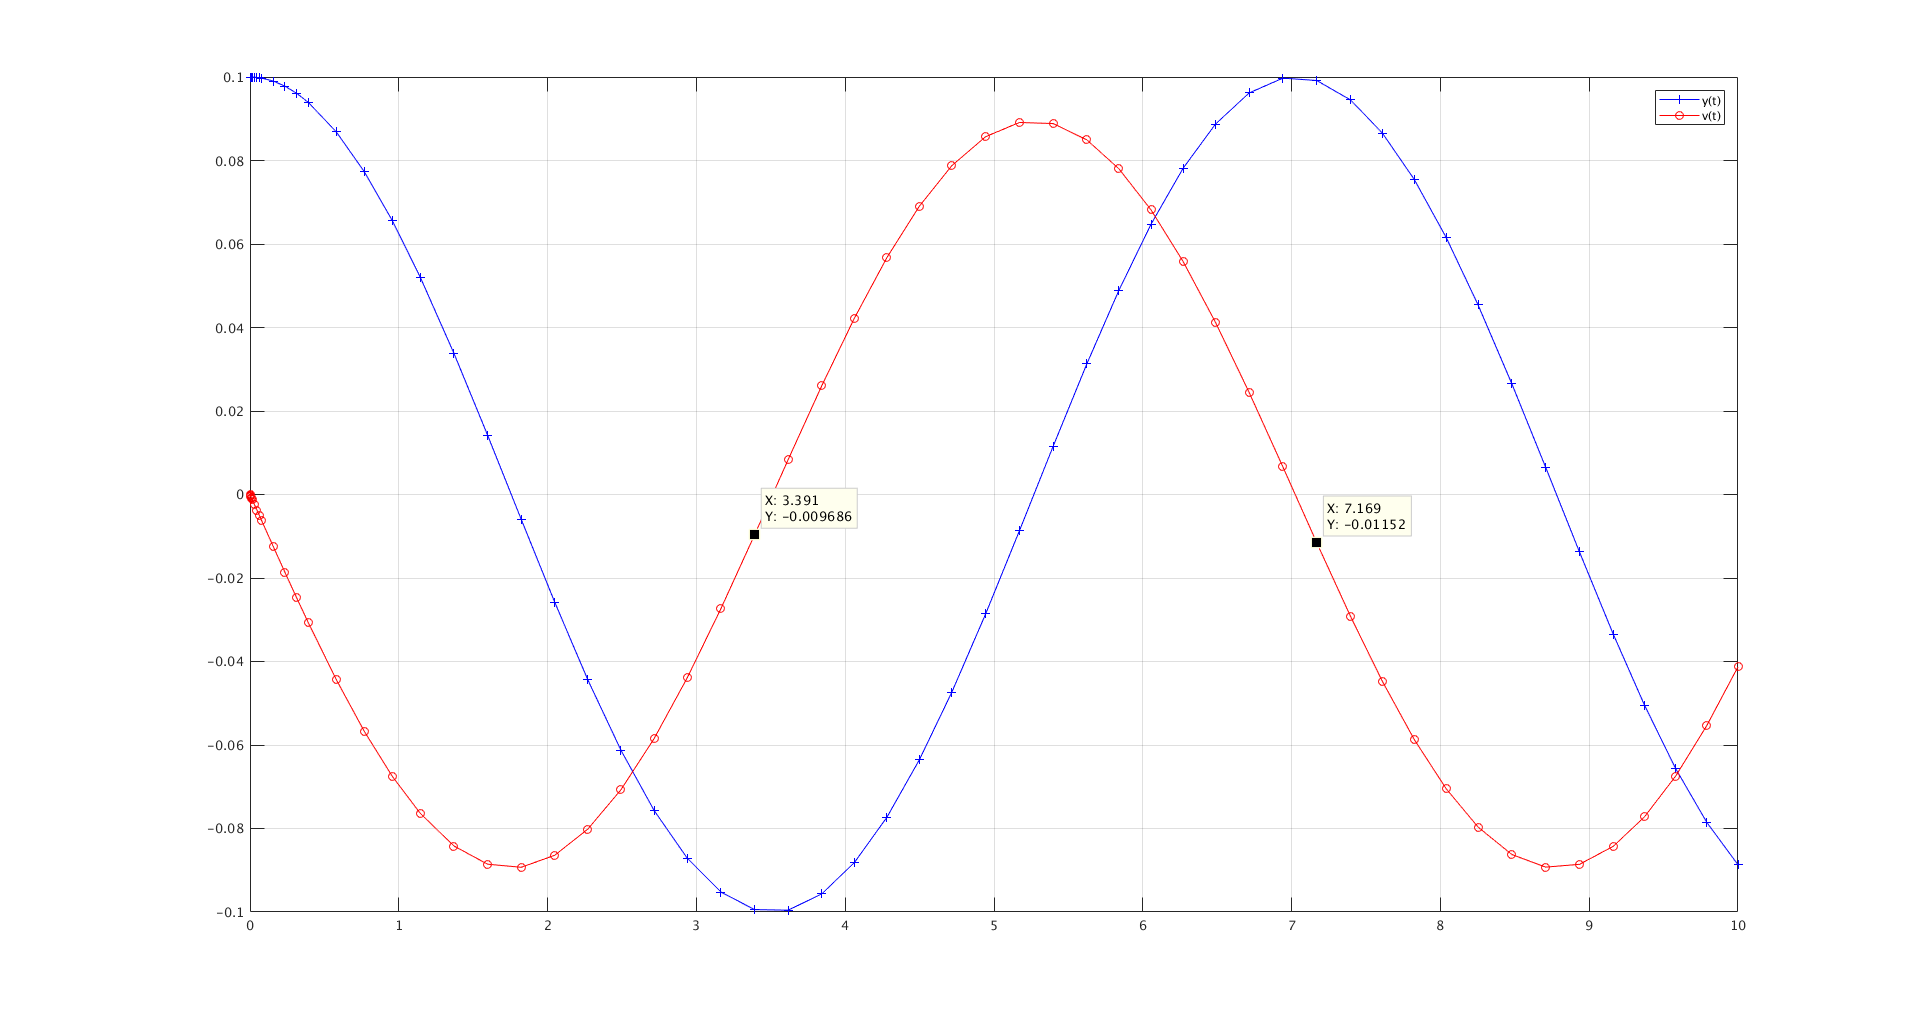
\includegraphics[scale=0.3]{1.png} \\
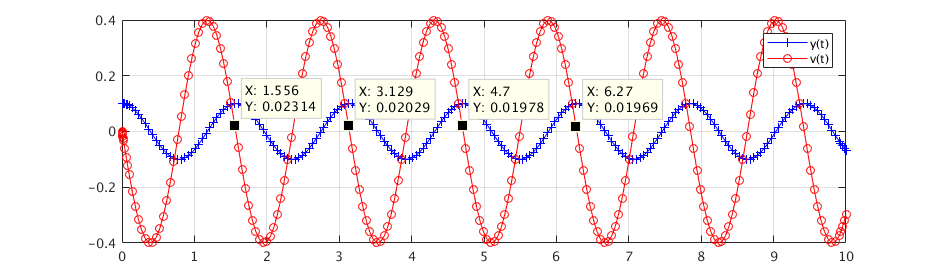
\includegraphics[scale=0.6]{2.png}

\end{itemize}
